\section{Auswertung}
\label{sec:Auswertung}

\subsection{Brennweitenbestimmung durch Messung von Gegenstands- und Bildweite}

In \ref{tab:brenn} sind die Werte für die Positionen des Gegenstandes $P_L$ und die Position des Schirms $P_S$ eingetragen.
Durch diese Werte lässt sich mit
\begin{equation}
  g=P_L-P_G
\end{equation}
die Gegenstandsweite ausrechnen.
Für die Bildweite gilt
\begin{equation}
  b=P_S-P_L
\end{equation}.
Auch die Größe des Bildes $B$ wurde gemessen.
Mit der Formel \ref{eqn:abbildung1} wird $V_1$ und mit \ref{eqn:abbildung2} wird $V_2$ berechnet.
Auch diese Werte, sowie die Differenz zwischen beiden, werden in Tabelle \ref{tab:brenn} hinzugefügt.
Die Brennweite der Linse wird mit \ref{eqn:brenn1} ausgerechnet und ebenfalls in die Tabelle eingetragen.

\begin{table}[H]
  \caption{Aufgeführt sind hier die gemessene Position der Linse, sowie die davon abhängige Position des Schirms um ein scharfes Bild zu erhalten.
  Zudem wurden aus diesen Werten Ggenstands- und Bildweite berechnet. Die Ungenauigkeit dieser Werte beträgt $\pm \qty{0.1}{\centi\meter}$.
  Dazu wurde die Größe des Bildes gemessen und einerseits mit den gemessenen Größen und andererseits mit Bild- und Gegenstandsweite der Abbildungsmaßstab berechnet.
  $\delta V$ ist die Differenz davon.}
  \label{tab:brenn}
  \centering
  \begin{tblr}{
    colspec={S[table-format=2.0] S[table-format=2.1] S[table-format=2.0] S[table-format=2.1] S[table-format=1.1] S[table-format=1.3] 
    S[table-format=1.3]  S[table-format=3.2]  S[table-format=1.1]},
    row{1}={guard, mode=math},
    }
    \toprule
    P_L \mathbin{/} \unit{\centi\meter} & P_S \mathbin{/} \unit{\centi\meter} & g \mathbin{/} \unit{\centi\meter} & b \mathbin{/} \unit{\centi\meter}
     & B \mathbin{/} \unit{\centi\meter} & V_1 \mathbin{/} \unit{\centi\meter} & V_2 \mathbin{/} \unit{\centi\meter} & A_V \mathbin{/} \unit{\percent} & f \mathbin{/} \unit{\centi\meter}\\
    \midrule
    40   &   65.9  &  15  & 25.9  &  5.0  & 1.667  & 1.727  &    3.60 &  9.498  \\
    45   &   64.0  &  20  & 19.0  &  2.9  & 0.967  & 0.950  &   -1.70 &  9.744  \\
    50   &   66.5  &  25  & 16.5  &  2.2  & 0.733  & 0.660  &  -10.00 &  9.940  \\
    55   &   70.2  &  30  & 15.2  &  1.8  & 0.600  & 0.507  &  -15.55 &  10.088 \\
    60   &   74.6  &  35  & 14.6  &  1.0  & 0.333  & 0.417  &   25.14 &  10.302 \\
    65   &   78.8  &  40  & 13.8  &  0.8  & 0.267  & 0.345  &   29.38 &  10.260 \\
    70   &   83.6  &  45  & 13.6  &  0.6  & 0.200  & 0.302  &   51.11 &  10.443 \\
    75   &   88.3  &  50  & 13.3  &  0.5  & 0.167  & 0.266  &   59.60 &  10.506 \\
    80   &   93.0  &  55  & 13.0  &  0.4  & 0.133  & 0.236  &   77.27 &  10.515 \\
    85   &   97.7  &  60  & 12.7  &  0.3  & 0.100  &  0.212 &  111.67 &  10.481 \\
    \bottomrule
  \end{tblr}
\end{table}

Für die Werte $P_L$, $P_S$ $g$, $b$ und $B$ ist der Ablesefehler $\pm \qty{0.1}{\centi\meter}$.
Der Fehler von $V_1$ und $V_2$ beträgt $\qty{0.033}{\centi\meter}$.

Der Mittwelwert der Brennweite beträgt $f \bar=\qty{10.178(0.335)}{\centi\meter}$.


In Abbildung \ref{fig:brenn} werden auf der x-Achse die gemessenen Werte für die Gegenstandsweite, und auf der y-Achse die Werte der Bildweite aufgetragen.
Die zueinander gehörigen Punkte werden verbunden und aus dem Schnittpunkt dieser Geraden wird die Brennweite bestimmt.
Diese sollte nämlich dem x und y Wert des Schnittpunktes entsprechen.

\begin{figure}[H]
  \centering
  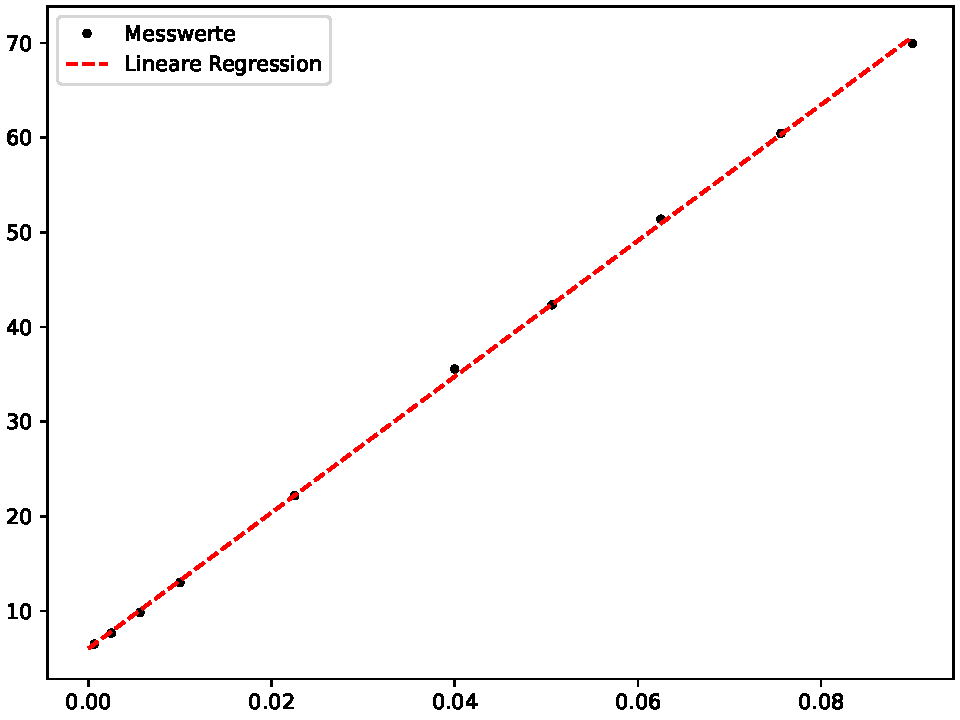
\includegraphics[height=7cm,width=14cm]{plot.pdf}
  \caption{Abgebildet sind die Werte der Bildweite auf der y-Achse und die der Gegenstandsweite auf der x-Achse.}
  \label{fig:brenn}
\end{figure}

In Abbildung \ref{fig:brenn} kann abgelesen werden, dass sich der Schnitpunkt bei $x=\qty{9(1)}{\centi\meter}$ und $y=\qty{11(1)}{\centi\meter}$ befindet.


